\chapter{Use Cases}
\label{chapter:usecases}
    
    Apart from a small impact and overhead on resources, OpenStack should also function reliably and as anticipated.
    Therefore, also advantages and new features have to be measured and evaluated.
    Considering the typical environment of OpenStack being, for example, a data center with usual hardware, embedded systems like automotive \acp{ECU} do not belong in this category.
    Nevertheless, OpenStack must perform reliable and consistent to benefit from its features and possibilities of Cloud Computing.
    As exemplary advantages of OpenStack in the context of automotive embedded systems, two scenarios are examined and measured.
    The following sections describe which value OpenStack can introduce through \ac{VM} distribution and migration.
    The measurements are performed using Python scripts to interact with the OpenStack cluster using the OpenStack Python SDK.
    All scripts used can be found at \cite{Malinowski2021}.
    
    
    \section{VM Distribution}
    \label{section:distribution}
        
        OpenStack enables the automatic distribution of \acp{VM} according to defined rules.
        While currently applications are bound to \acp{ECU}, they cannot be executed elsewhere.
        However, this would come in handy if, for example, an individual \ac{ECU} is highly loaded while another does not have much to process.
        By pooling the available resources and distributing them, \acp{VM} can be executed independently on the most suitable hardware.
        The functionality should work as intended, otherwise, unforeseeable complications could occur, leading to, for example, overloaded \acp{ECU}.
        
        \noindent The distribution on those platforms is evaluated separately because of specific instruction sets and, therefore, specific images for the ARM and x86 nodes.
        The Nova-Scheduler being responsible, among other things, for the assignment of \acp{VM} to hosts, can be configured by various parameters.
        For the evaluation of \ac{VM} distribution, the following parameters are modified.
        
        \newpage
        \begin{itemize}
            
            \item \textsl{scheduler\_driver\_task\_period} \hfill \\ 
            This parameter sets the interval of how often the scheduler updates its resource information.
            A smaller interval means better and more accurate values but also an increased overhead as the information must be polled more often from the compute nodes.
            
            \item \textsl{cpu\_weight\_multiplier} \hfill \\ 
            This parameter sets the importance of used \ac{CPU} cores.
            A positive multiplier will try to achieve even distribution with an even number of cores used on every host.
            A negative multiplier will first use all available cores on one compute node before utilizing the next one.
            
            \item \textsl{ram\_weight\_multiplier} \hfill \\ 
            This parameter sets the importance of used memory.
            A positive number will try to achieve even memory utilization on all hosts. In contrast, a negative number will try to first utilize all available memory on one host before moving on to the next one.
            
            \item \textsl{disk\_weight\_multiplier} \hfill \\ 
            Similar to the cpu\_weight\_multiplier and ram\_weight\_multiplier, this parameter sets the importance of disk utilization.
            A positive number will again try to distribute VMs evenly based on the hosts' disk usage, while a negative number will first stack the VMs on one host. 
            
            \item \textsl{build\_failure\_weight\_multiplier} \hfill \\ 
            This parameter describes how much build failures of \acp{VM} on hosts influence the \ac{VM} assignment.
            The higher the value specified, the more build failures weigh, resulting in hosts with recent build failures not being chosen for a new \ac{VM} in the first place.
            
            \item \textsl{io\_ops\_weight\_multiplier} \hfill \\ 
            Like the previous weight\_multipliers, this parameter considers the \ac{CPU} usage on the compute nodes.
            If a positive value is defined, compute nodes with high \ac{CPU} utilization will be chosen over ones with low utilization.
            On the other hand, a negative value configures the scheduler to chose low-utilized nodes over high-utilized ones.
            
        \end{itemize}
        
        
        \subsection{Distribution Scenarios}
        
            On both platforms, two different and contrary distribution strategies are tested.
            First, an equal distribution regarding the \ac{CPU} cores is tried to be achieved.
            As the CPU cores are one source of computational performance, equal distribution among all compute nodes would decrease each compute node's CPU load.
            This would prevent the \ac{VM} performance from being degraded due to the host being too highly loaded.
            Second, a stacked distribution regarding the \ac{CPU} cores is tried to be achieved.
            Configuring the scheduler to first use all available \ac{CPU} cores on one compute node until utilizing a second node would enable to set these nodes into a standby or low power mode.
            Due to this, energy could be saved as not all nodes would be necessarily utilized all the time.
            Table \ref{table:distribution_parameters} shows the parameter configurations for both distribution strategies.
            
            \begin{table}[ht]
                \begin{center}
                    \begin{tabular}{l|c|c}
                        \textbf{\makecell[c]{Parameter}} & \textbf{Stacked Distribution} & \textbf{Equal Distribution} \\
                        \noalign{\hrule height 1.5pt}
                        scheduler\_driver\_task\_period 		&	5		&	5 \\
                        cpu\_weight\_multiplier			&	5.0		&	-5.0 \\
                        ram\_weight\_multiplier 			&	5.0		&	-5.0 \\
                        disk\_weight\_multiplier			&	5.0		&	-5.0 \\
                        build\_failure\_weight\_multiplier		&	5.0		&	0.0 \\
                        io\_ops\_weight\_multiplier 		&	-1.0		&	5.0
                    \end{tabular}
                \caption{Nova-Scheduler parameters for VM distribution}
                \label{table:distribution_parameters}
                \end{center}
            \end{table}
            
            \noindent The \ac{VM} flavors used are the smallest defined, being the \textsl{rcar-01-128-06} and the \textsl{xeon-06-21504-106} flavor.
            In order to best evaluate the distribution, as many \acp{VM} as possible should be spawned and distributed.
            With the ARM cluster having only 16 cores in total, this was the highest number of machines possible.
            To keep the Xeon cluster comparable and the testing time reasonable, it was also decided to spawn 16 machines.
            Therefore the flavors representing one-eighth of the total resources were chosen.
            
            \noindent The scenario measurements are performed in the following way:
            On each cluster, 16 \acp{VM} are created and started sequentially.
            For every \ac{VM}, during its creation, the \ac{VM}'s compute host is checked.
            This way, the initially scheduled host by the Nova-Scheduler is captured, as well as any host changes due to build failures.
            The scenario is performed one time with each scheduler configuration.
        
        
        \subsection{Scenario Evaluation}
            \begin{figure}[ht]
              \centering
              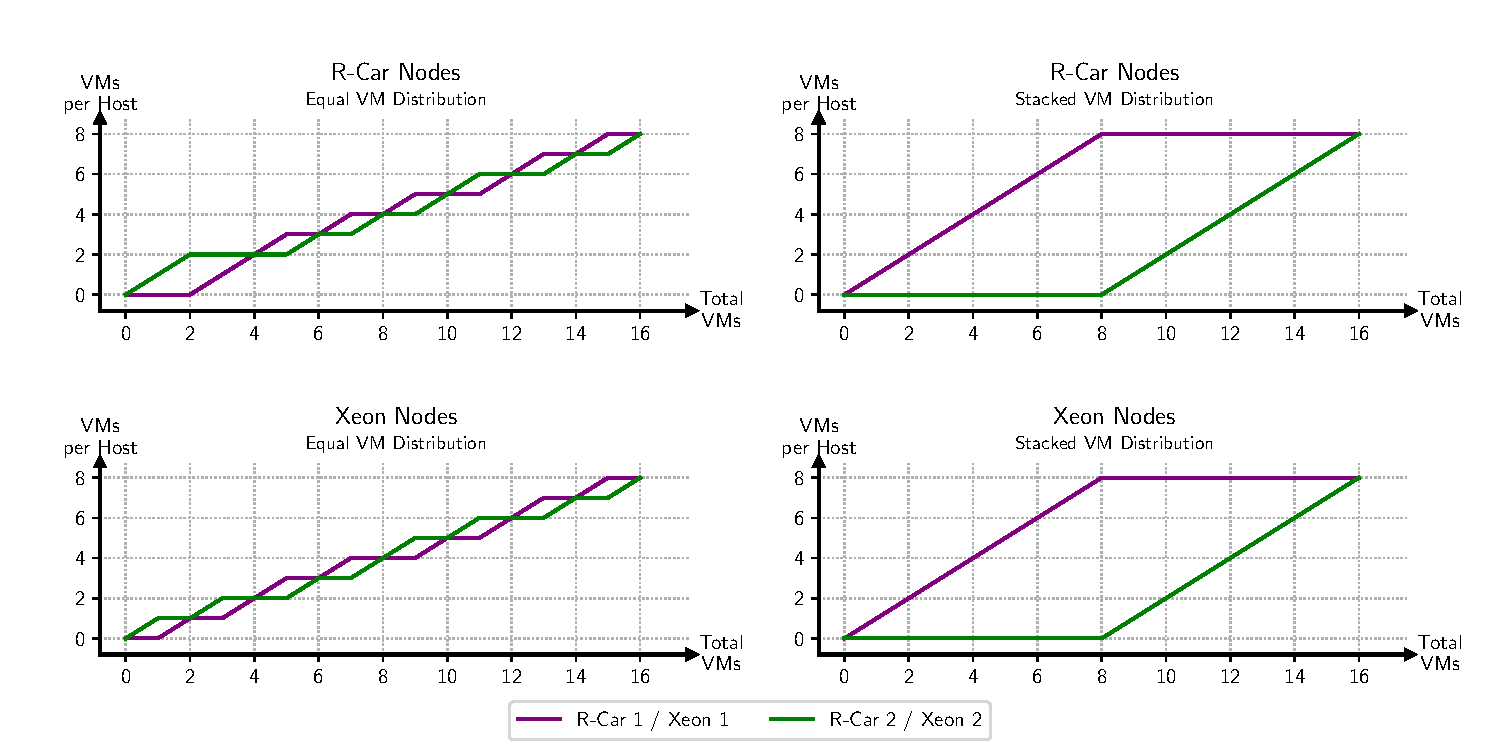
\includegraphics[width=\linewidth]{06_all-distribution.pdf}
              \captionof{figure}{VM distribution across compute nodes}
              \label{fig:vm_distribution}
            \end{figure}
            
            \noindent Figure \ref{fig:vm_distribution} shows the \ac{VM} distribution across the R-Car cluster (top row) and the Xeon cluster (bottom row).
            First and foremost, no errors or host reschedules are visualized in the plots as no errors or reschedules occurred.
            For all distributions and hosts, the spawning was always successful.
            Further, it is clearly visible in the figure that the different distribution scenarios worked and were realized as expected by the Nova-Scheduler.
            
            \noindent The right column of Figure \ref{fig:vm_distribution} shows the stacked distribution.
            The first eight VMs are clearly assigned to the R-Car 1 / Xeon 1 compute node, while the last eight VMs are assigned to the other compute node.
            The left column shows the equal \ac{VM} distribution. 
            Obviously, over time the \acp{VM} are distributed equally across the two nodes.
            On the R-Car cluster as well as on the Xeon cluster, the distribution is not strictly alternating during the equal distribution, depicted by the first two \ac{VM} assignations to the R-Car 1 node.
            Also, the 10th and 12th \ac{VM} are assigned to R-Car 1 in a row.
            Similar behavior can be seen on the Xeon cluster: \acp{VM} 4 and 5, 8 and 9 and 12 and 13 are assigned to the same compute node in a row.
            However, as the number of running \acp{VM} per host is the same, a selection of the same hosts twice in a row is not false, as both hosts are equally utilized.
            
            \noindent The correct functionality of the \textsl{io\_ops\_weight\_multiplier} is captured in the first \ac{VM} assignment on the Xeon cluster to the Xeon 2 node.
            Xeon 1, being the controller, is more utilized, and therefore Xeon 2 is chosen over Xeon 1.
            However, striking are the first two \ac{VM} assignments to the R-Car 2 node using an equal distribution (Figure \ref{fig:vm_distribution}, top-left plot). 
            Assigning the second \ac{VM} also to the R-Car 2 node indicates that the \ac{CPU} of R-Cars 1 is higher utilized at that time, as it has to outweigh the \ac{CPU}, memory, and disk multiplier.
            However, the third and fourth \ac{VM} are assigned to the R-Car 1 again, balancing the distribution again.
            
            \noindent Concluding, both scenarios show that a distribution strategy on embedded hardware for \acp{VM} is possible.
            Also, the absence of reschedules and build errors demonstrates the reliable operation of OpenStack.

        
    \section{VM Migration}
    \label{section:migration}
  
        \noindent A large number of \acp{ECU} in today's vehicles brings two essential advantages.
        The presence of multiple \acp{ECU} brings redundancy and enables to group functionality on particular \acp{ECU}.
        In case of an \ac{ECU} failure, another \ac{ECU} can continue its work to avoid security and safety implications.
        Similarly, real-time software can be separated from less time-critical software to avoid interference or performance degradation.
        While the separation or grouping can be achieved easily and with various OpenStack methods, the aspect of redundancy can also be satisfied by OpenStack.
        Similarly, multiple \acp{VM} could calculate the same task on different hosts in parallel, realizing today's approach.\\
        Yet, OpenStack further enables a different approach to deal with, for example, instance failures.
        By executing all functionality inside \acp{VM}, these \acp{VM} are decoupled from the hardware and can be migrated to other hosts.
        This can happen by transferring a switched-off instance but also a live, currently active instance.
        Therefore, if an \ac{ECU} being a compute host fails or a problem is detected, its \acp{VM} can be migrated to other running hosts. 
        As valuable as live-migration might sound, the performance during it must not be impacted too much to provide value, and the duration must be reasonable.
        While \acp{VM} are shifted to another compute host, the resources are in a state without one single defined host.
        As the resources are either partly on two hosts or for a short time on neither host, the performance could suffer drastically.
        Also, depending on the resources used by the \acp{VM}, the duration could take an unacceptable amount of time.
   
   
    \subsection{Time}
    \label{subsection:usecases_time}

        \noindent To evaluate the live-migration duration of \acp{VM}, a Python script is executed.
        The script boots a \ac{VM} on one host and flowingly migrates it to another host.
        Same as the \ac{VM} distribution, the migration time is evaluated separately for the R-Car and the Xeon cluster. 
        Using the OpenStack Python SDK, the VM's status is periodically polled, and the interval between entering and leaving the \textsl{migrating}-status is used for evaluation.
        To ensure the instances are migrated between the right hosts, only the compute services on the relevant hosts are active during the migration.
        The migrations are performed with all configured flavors in order to discover potential impacts of resources on time.
        
        \subsubsection*{Time - Evaluation}
        
            \begin{figure}[H]
              \centering
              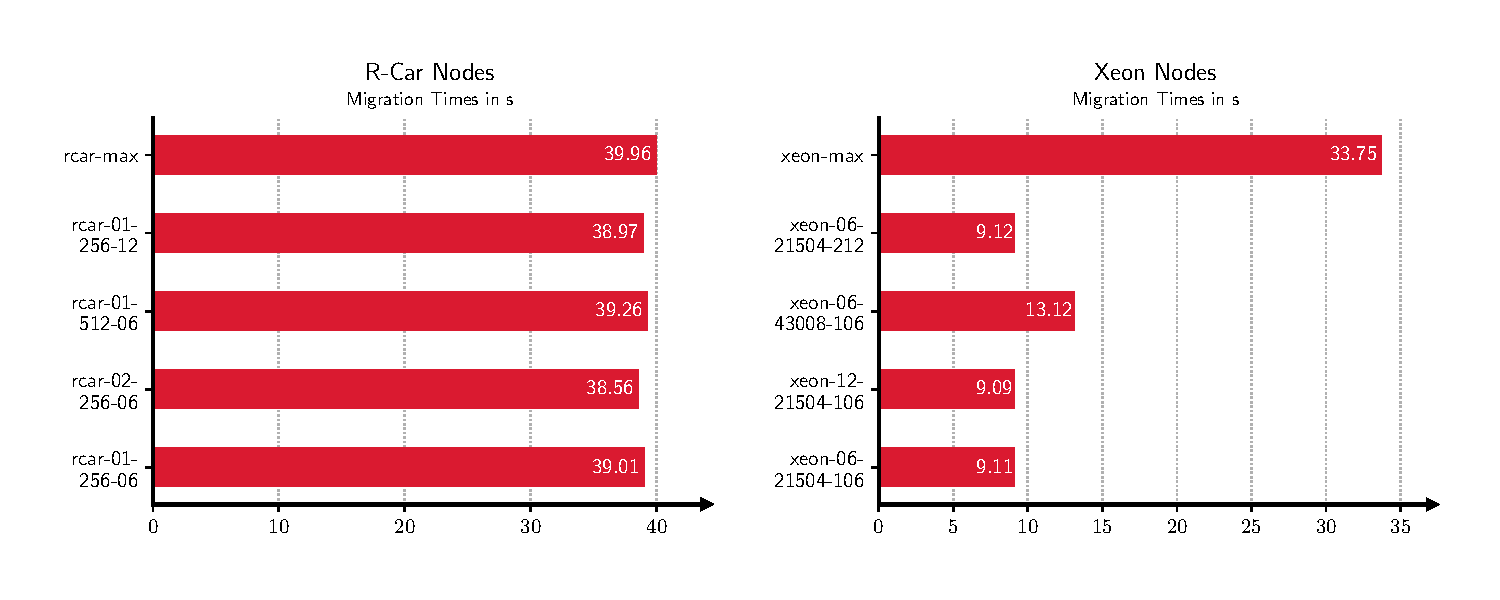
\includegraphics[width=\linewidth]{06_all-migration.pdf}
              \captionof{figure}{VM migration times}
              \label{fig:vm_migration_time}
            \end{figure}
            
            \noindent Figure \ref{fig:vm_migration_time} shows the migration times for the R-Car and Xeon cluster.
            While on the R-Car nodes, all flavors take about 40 seconds to migrate, on the Xeon nodes, the flavors need about 10 seconds, except the \textsl{max}-flavor taking about 34 seconds.\\
            Considering the Xeon migration times, one resource can be identified as exceptionally time-consuming.
            All flavors except the \textsl{max}-flavor represent a twofold increase of one resource compared to the smallest flavor \textsl{xeon-06-21504-106}.
            Neither double the CPU cores nor double the disk size seems to affect the migration time significantly.
            Double the memory, however, extends the migration time by three seconds.
            Considering now the \textsl{max}-flavor needing 34 seconds together with the fact that a memory increase of 21504 MB increases the duration by three seconds, memory seems to have the most significant impact.
            Therefore, for the total migration time of the \textsl{max}-flavor, 24 seconds (8*3 seconds) are necessary only to migrate the memory, while the remaining resources need ten seconds in total.\\
            Due to the \acp{VM} being in an idle state, neither the \ac{CPU} nor the memory or the disk is utilized.
            This explains why neither resource increase is directly reflected in an increased migration time.
            As the actual amount of resources to migrate stays the same, no actual increase in resource usage is present, and therefore no change is introduced.
            However, while the memory utilization is also not differing from flavor to flavor, it nevertheless has an impact, leading to the conclusion that the memory has to be freed on the old host and allocated in some way on the new host.
            
            \noindent Using these conclusions, the overall low performance and the little to no variation in migration time on the R-Car cluster can be explained.
            Striking, no substantial difference in migration time between the smallest, the biggest, or any other flavor can be identified.
            Also, a substantial influence of the memory size is absent.
            This suggests that the migration time is mainly influenced by something else.
            Considering the fact that all \acp{VM}, on the Xeon and on the R-Car nodes, where started using local storage, everything is existing and stored locally on the current host.
            Flowingly, everything has to be transferred to the destination host accordingly during the migration. 
            On the one hand, this explains the not changing migration times on the Xeon Cluster with increased storage because the actual data size stays the same.
            On the other hand, the Xeon nodes are connected via a 10 Gbit Ethernet connection, while the R-Car nodes have only a 1 Gbit connection.
            This leads to the fact that no variation in migration on the R-Car cluster can be identified because the storage migration always influences the migration time the most.
            Having a ten-times slower connection and less powerful hardware, the storage migration takes more time than anything else.
            
            \noindent In current vehicles, 1 Gbit Ethernet connections are already present, and using 10 Gbit capable hardware will be the next step to follow.
            Together with powerful hardware, reasonable migration times can be achieved.
            Taking into account that memory requirements, as well as storage requirements, are kept as low as possible in embedded software, the performance would further increase.
            However, a utilized CPU and memory might additionally impact the migration time, as examined in the next section. 
        
        
    \subsection{Performance}
    \label{subsection:usecases_performance}
    
            \noindent Considering live-migration in a redundancy use case, besides the reliability and the migration time, the performance during it is critical.
            Depending on the use case and its requirements, either continuation or performance or both may be favored.
            For example, in a time-critical real-time software, the performance must not be impacted, as this would make the application indeterministic and could lead to catastrophic events.
            In the case of an application with less strict timing requirements like an infotainment application, however, the functionality's continuation is more important, even if the performance is slightly reduced for a short amount of time.
            
            \noindent The \ac{CPU} being the primary computational resource, it was decided to gather values about the \ac{CPU} performance.
            In order to achieve this, the \textsl{Sysbench} benchmark\footnote{Sysbench Benchmark: https://github.com/akopytov/sysbench} is used.
            The benchmark uses prime number factorization to determine \ac{EPS} and latency values of the \ac{CPU}.
            Considering these values over time during a live-migration, a statement about the performance is possible.\\
            The values are collected as follows:
            First, a \ac{VM} is created, and all software updates inside it are performed.
            Next, the Sysbench benchmark is installed using aptitude.
            The Sysbench benchmark is configured to factorize as many prime numbers as possible for one second, every two seconds.
            The flavor with the doubled \ac{CPU} core number is used on both clusters, and the number of threads used by Sysbench is specified to be half the number of available cores.
            This provides \ac{EPS} and latency values every two seconds so that a complete visualization of the migration performance can be established without losing any significant values.
            The \ac{VM} is run for 2 minutes on one compute host and flowingly migrated to the other host in its cluster.
            This is performed four times so that four migrations are captured.
        
        
        \subsubsection*{Performance - Evaluation}

            \noindent Figure \ref{figure:vm_migration_performance} shows the collected values.
            Visible in both clusters are the \ac{EPS} drop and the latency spike during the migrations.
            However, the absence of a definite plateau in the \ac{EPS} and latency plot indicates no measurement values were lost, and the impact only lasts a short amount of time.
            Further, both clusters' migration durations increase compared to the results in Figure \ref{fig:vm_migration_time}.
            On the R-Car cluster, using the \ac{VM} flavor \textsl{rcar-02-128-06}, the migration time increases from 40 seconds to 100 seconds (best case) or 150 seconds (worst case).
            Similarly, on the Xeon cluster, using the \ac{VM} flavor \textsl{xeon-06-21504-106}, the migration time increases from 10 seconds to 17 seconds (best case) or 30 seconds (worst case).
            This clearly shows that a non-idle \ac{VM}, having a utilized \ac{CPU} takes longer to migrate than an idle \ac{VM}.
            Additionally, Figure \ref{figure:vm_migration_performance} shows that Xeon 1, in general, achieves lower EPS and higher latency values running the core services.
            
            \begin{figure}[H]
                \centering
                \begin{subfigure}[b]{\textwidth}
                    \centering
                    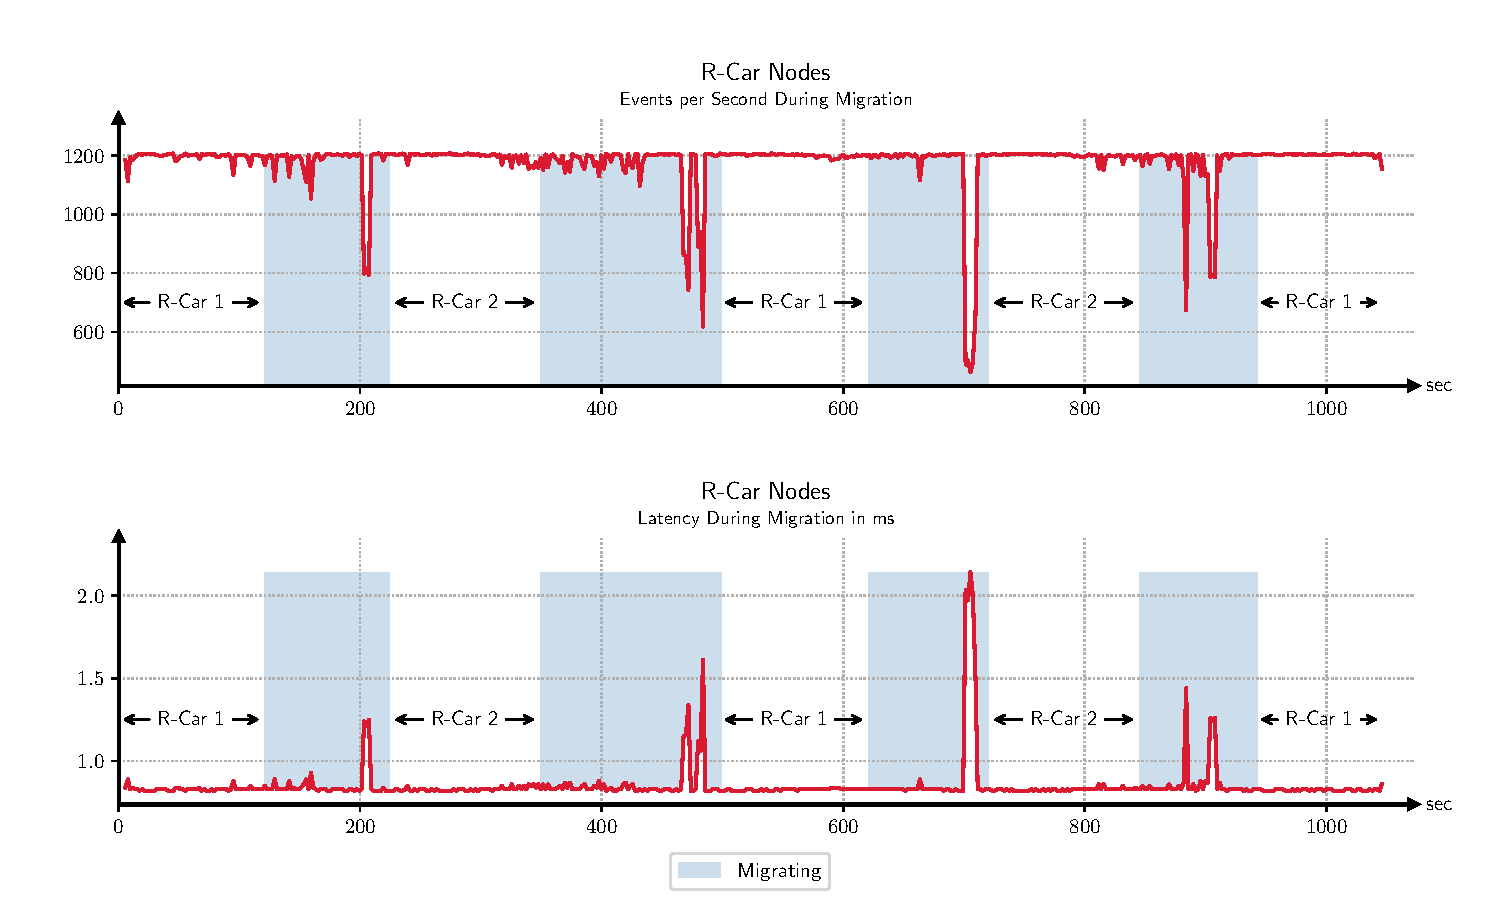
\includegraphics[width=\textwidth]{06_rcar_cluster_migration_performance.pdf}
               \end{subfigure}
               \caption[]{VM migration performance on the R-Car and Xeon cluster}
            \end{figure}%
            \begin{figure}[ht]\ContinuedFloat
                \centering
                \begin{subfigure}[b]{\textwidth}
                    \centering
                    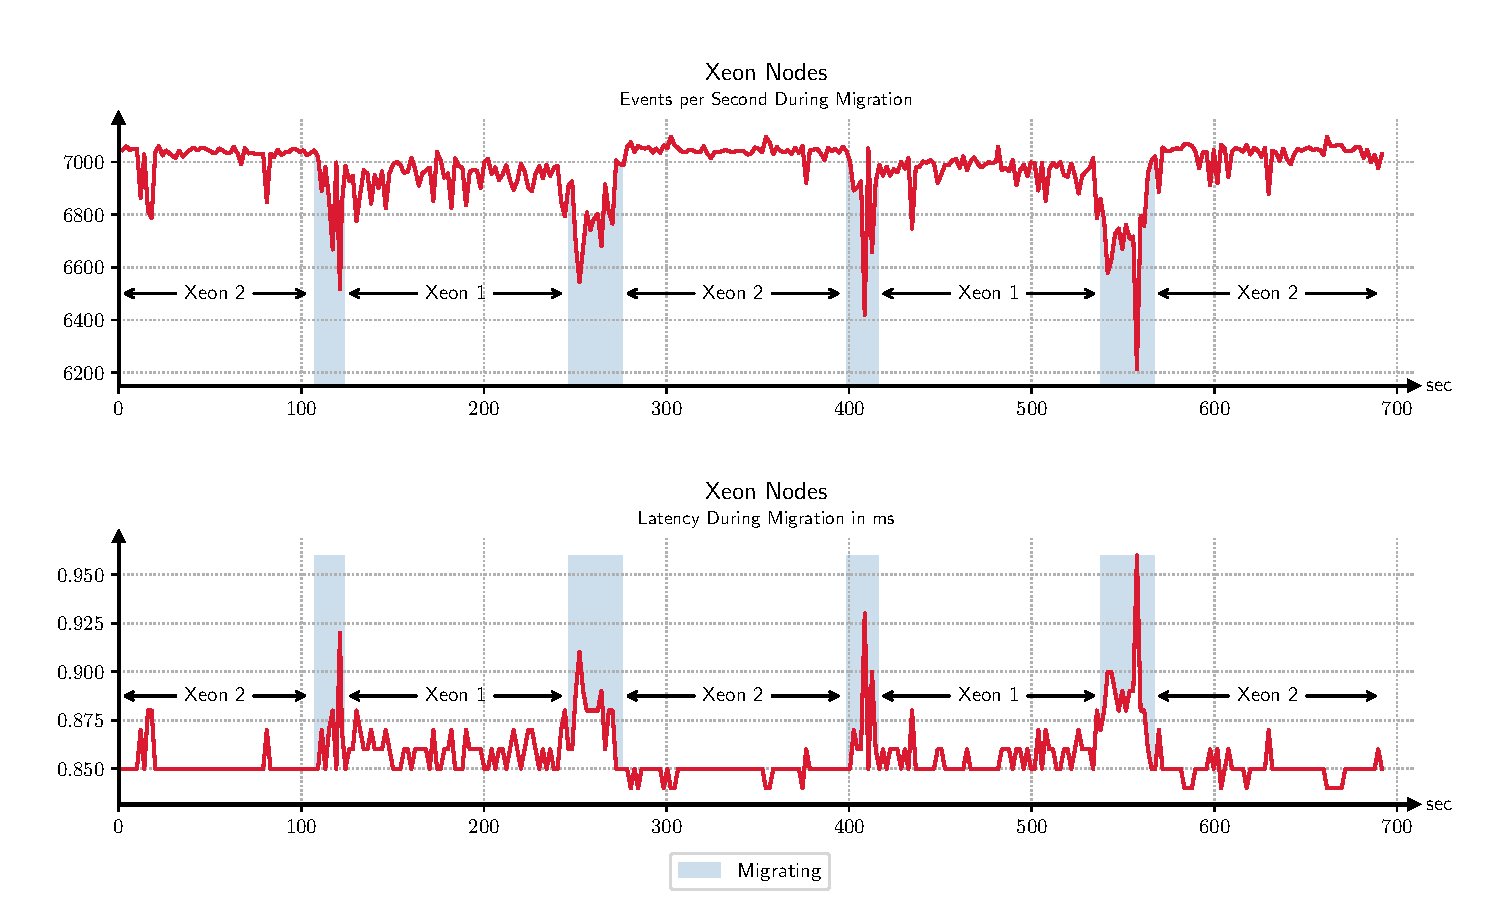
\includegraphics[width=\textwidth]{06_xeon_cluster_migration_performance.pdf}
                \end{subfigure}
                \caption[VM migration performance on the R-Car and Xeon cluster]{VM migration performance on the R-Car and Xeon cluster (cont.)}
                \label{figure:vm_migration_performance}
            \end{figure}

            \noindent Examining the plot in detail, it can be seen that the performance degradation, in general, is only given for a concise amount of time, even when the migration itself takes much longer.
            The peak EPS drops only last for a couple of seconds on the R-Car and the Xeon nodes.
            This is very noticeable on the R-Car nodes.
            Due to only executing one thread on the R-Car nodes, only when this specific thread or rather \ac{CPU} core is migrated, the \ac{EPS} number drops.
            Nevertheless, the drop from 1200 \ac{EPS} to 800-520 \ac{EPS} corresponds to a performance degradation of 33-52\%, being non-negligible even in short time frames if performance is critical.\\
            On the Xeon nodes, the degradation is not as significant as on the R-Car.
            Due to executing three threads, the peak performance drops during the migration are less significant.
            On the Xeon nodes, the performance drops by 400-800 \ac{EPS}, corresponding to a 5-10\% performance impact.
            This leads to the finding that multi-threaded processes and parallelized applications suffer lower performance degradation during a live-migration compared to single-threaded processes.
            As threads seam to be migrated one after another, improved fundamental performance through more threads or higher single-core performance lowers the percentage degradation.
            
            \noindent Considering the latency, the spikes correspond precisely to the \ac{EPS} drops.
            Reasonably, the EPS number drops if the CPU has a higher latency, meaning that fewer requests can be carried out per time frame if the CPU takes longer to react to a request.
            However, the R-Car latency spikes are much higher (2 milliseconds) compared to the Xeon spikes (0.1 milliseconds).
            This can be attributed to the fact that first, the Xeon \ac{CPU} is more powerful, and second, executing three threads leads to a high probability of some thread always reacting quickly to a request.
            The influence of multiple threads can be seen in the fact that the time interval in which the \ac{EPS} number drops is much longer compared to the R-Car cluster.
            While on the Xeon cluster the performance degradation is present for a longer duration, the R-Car cluster suffers a higher but shorter degradation.
            Nevertheless, on both clusters the rise in \ac{CPU} latency inhibits a usage for real-time applications, as the CPUs' responsiveness becomes indeterministic. 
            
            \noindent Further, the graphical representation of the migration confirms the previous section's statement regarding the time share of different resources.
            The figure shows that the \ac{CPU} is migrated last as the spikes and drops appear at the end of the migration.
            Especially, the R-Car plot shows that the \ac{CPU} migration happens in a concise time frame compared to the total duration. 
            As the total duration increases in contrast to the previous section, the memory impact on the migration time is further hardened.
            The CPU and memory utilization being the only difference to the measurements in Section \ref{subsection:usecases_time}, their utilization can be made responsible for the longer migration time.
            
    
    \subsection{Application Migration}
    \label{section:usecases_application}
        
        Having examined the migration time and performance in the previous sections, an actual application shall be migrated.        
        Since real-time and hard-safety applications would require further and more complex tests, these are out of this thesis's scope.
        Nevertheless, the previous measurements and scenarios suggest that an OpenStack cluster on automotive hardware is realizable.
        To demonstrate this, it was decided to evaluate the migration of a Tetris application.
        Being a small game, this represents the use case of playing a game on a vehicle's infotainment system.
        Not having hard real-time requirements but mainly regarding the quality of service, this reflects the previously described choice of a continuous function over high performance.
        However, the performance should still be as good as possible.

        \noindent This use case is evaluated in a similar manner as the migration performance in the previous section.
        However, as the Tetris game requires a more sophisticated user interface, the VMs must be prepared accordingly.
        A desktop shall represent the user interface which would also be present in an actual infotainment system.
        As the Ubuntu Cloud Images do not initially include a desktop, it first has to be installed.
        Further, a \ac{VNC} server is installed inside the \ac{VM}.
        This enables the remote access of the machine's desktop and its interaction.
        As Tetris game, the game \textit{Quadrapassel}\footnote{Quadrapassel Game: https://wiki.gnome.org/Apps/Quadrapassel} from the Ubuntu repository was chosen due to its easy installation via aptitude and low hardware requirements.\\
        In order to evaluate this scenario, two different measurements are performed.
        First, using the resource usage measurements from Section \ref{section:methodology_idle}, the overhead and resource usage with an active application inside the \ac{VM} are examined.
        Second, the same measurements are performed during the live-migration.
        Only one migration is measured as multiple migrations do not provide more information but only extend the test time.
        
         \subsubsection*{Application Resource Usage - Evaluation}
        
            \noindent Before the migration, Figure \ref{figure:use_case_usage} shows the resource usage on the compute hosts R-Car 2 and Xeon 2.
            In addition to the tests from Section \ref{section:evaluation_consumption}, in this measurement, the \acp{VM} are not left idle after creation, but the \ac{VNC} server and the application are started.
            Figure \ref{figure:use_case_usage} enables a clear distinction between the different actions performed while preparing the system before migration. 
            In addition, to Figure \ref{fig:all_idle}, through measuring the \ac{CPU} and memory usage inside the \ac{VM} too, even better visualization of OpenStacks overhead is possible.
            Regarding the R-Car node, an overhead of 2\% in \ac{CPU} usage and an overhead of 100 MB in memory usage is found.
            For the Xeon node, the \ac{CPU} overhead also lies between 1-2\% during an active application, while the memory overhead lies at about 4 GB.
            Also visible, the \ac{CPU} and memory usage only rise significantly if the usage inside the \ac{VM} rises, apart from small periodic peaks due to periodic OpenStack processes.
            Further, the figure shows the difference between the \ac{VM} startup and the OS's actual boot inside the \ac{VM}.
            On the R-Car cluster, the duration between the \ac{VM} startup and the actual \ac{VM} boot is significantly longer than on the Xeon cluster.
            As explained in Section \ref{section:evaluation_consumption}, this originates from the higher computational power of the Xeon platforms.
            
          
        
       
        \subsubsection*{Application Migration - Evaluation}
            
            \noindent Figure \ref{figure:use_case_migration} shows the \ac{CPU} and memory usage on the R-Car and Xeon hosts during the live-migration.
            First and foremost, the live-migration succeeds.
            The player is able to continue to play the game throughout the whole migration without significant interruption.
            The game lags for a couple of seconds only towards the end of the migration, leading to inputs from the keyboard and outputs from the screen being slightly delayed.
            This fits together with the gained knowledge on the performance during a live-migration.
            As the performance drops towards the end, also the game performance drops.
            However, the game is not interrupted entirely and is available throughout the migration.
            
            \begin{figure}[H]
                \centering
                \begin{subfigure}[b]{\textwidth}
                    \centering
                    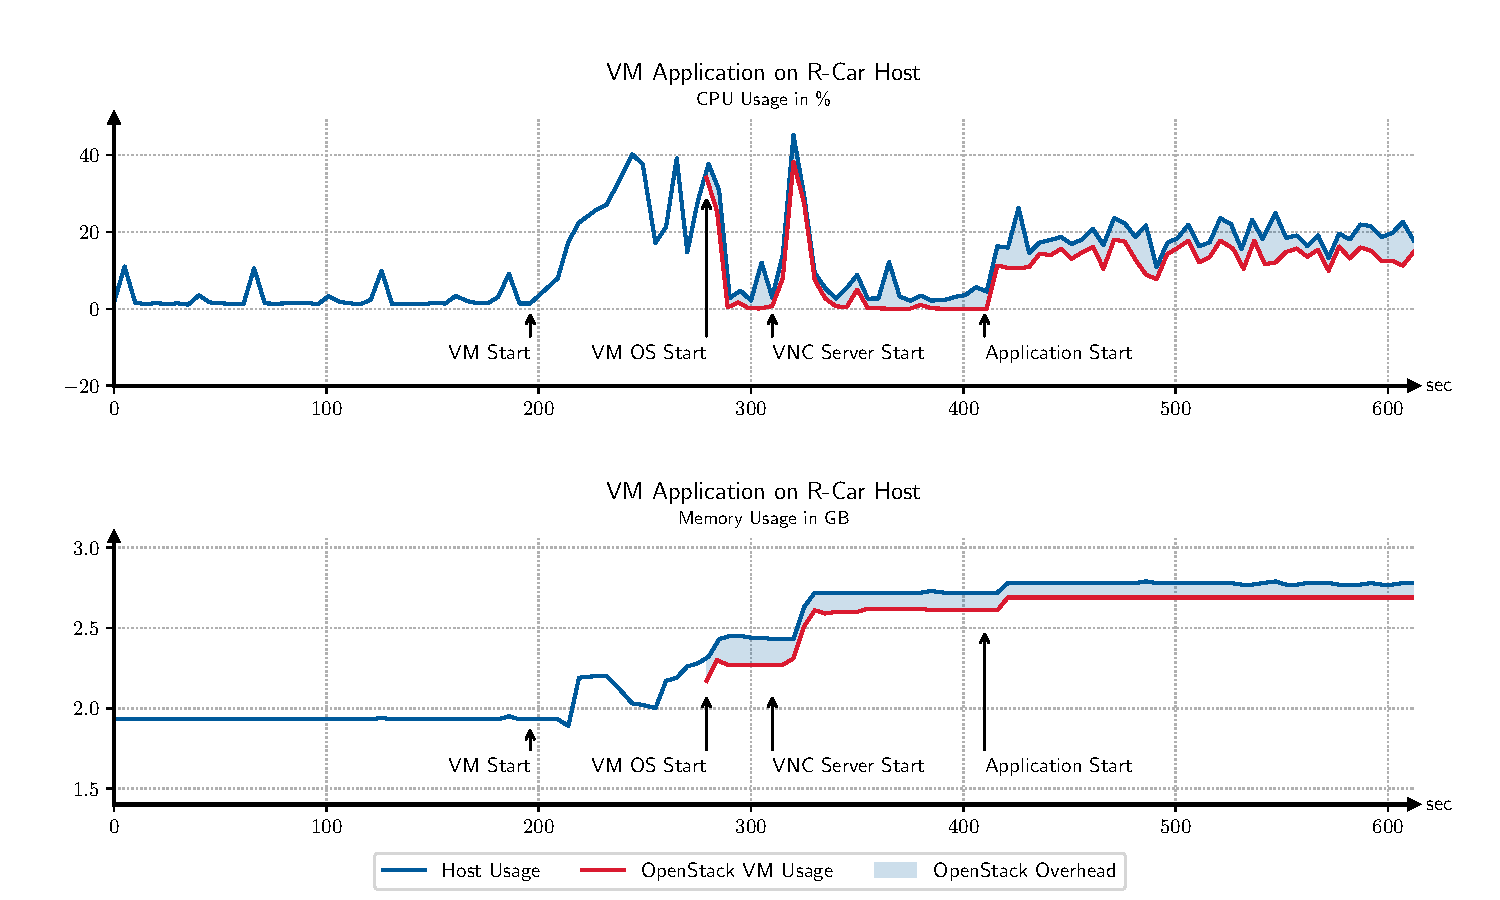
\includegraphics[width=\textwidth]{06_use-case-usage-rcar.pdf}
                \end{subfigure}
                \begin{subfigure}[b]{\textwidth}
                    \centering
                    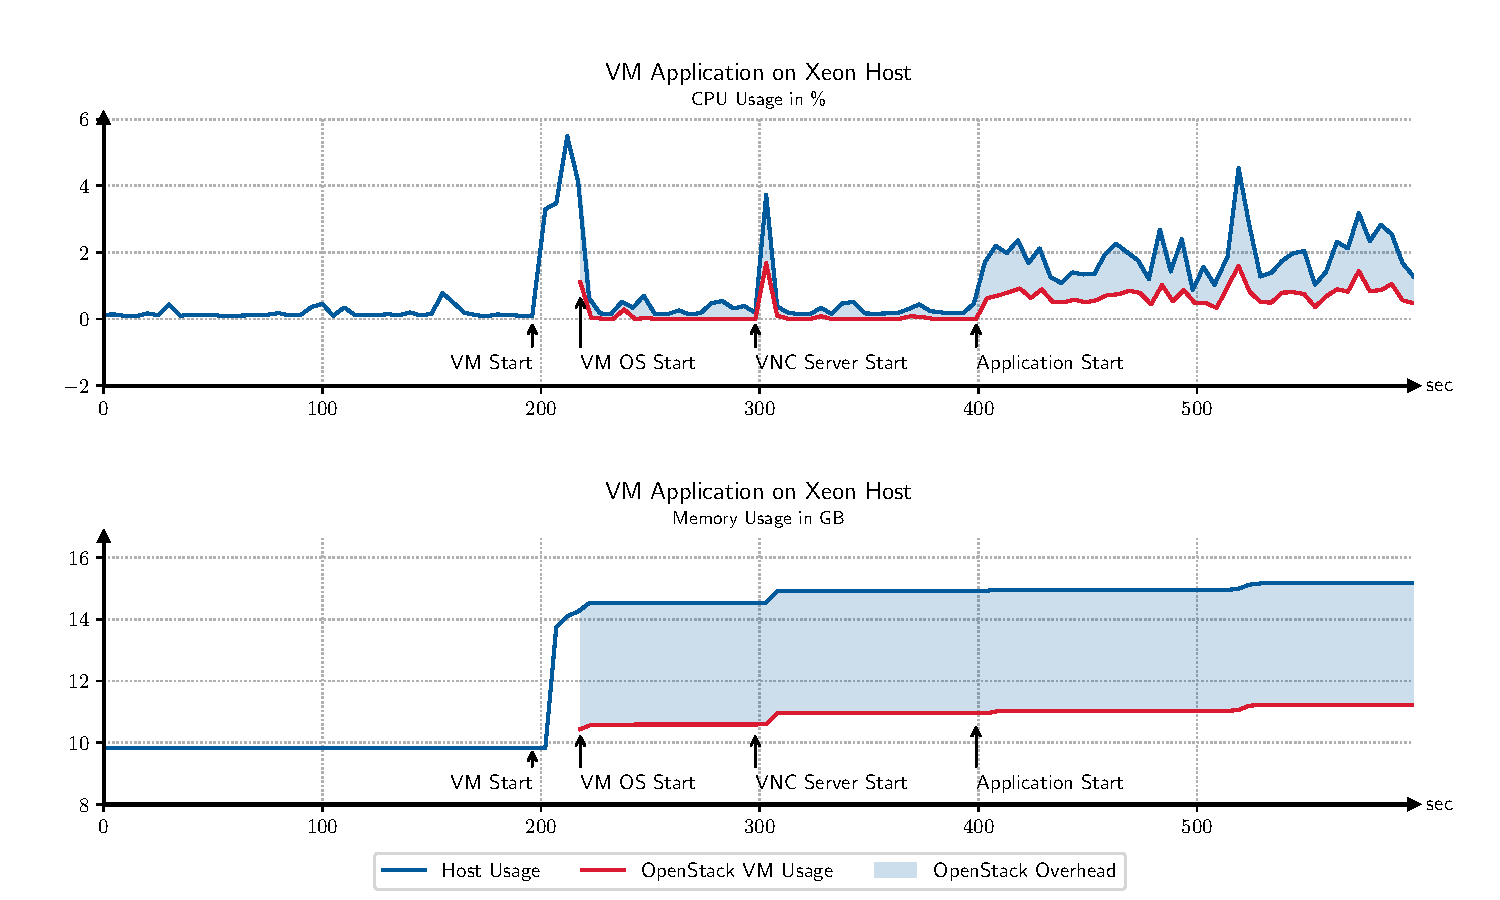
\includegraphics[width=\textwidth]{06_use-case-usage-xeon.pdf}
                \end{subfigure}
                \caption{R-Car and Xeon resource usage with VM application}
                \label{figure:use_case_usage}
            \end{figure}
            
            
            \noindent Examining the results in detail, the R-Car cluster duration shows as most striking.
            Taking about 1850 seconds or 31 minutes, it is significantly higher compared to the duration measured in Section \ref{subsection:usecases_time} and \ref{subsection:usecases_performance}.
            However, this is due to the limited resources on the R-Car.
            The measured memory values show that the use case requires 3.5-3.6 GB of memory, which corresponds to the R-Car's maximum available memory.
            As from this point on, the swap-memory is used, the operations are much slower, resulting in a significantly longer migration duration.
            As the disk data has to be migrated too, it first has to be read into memory before transferring it over the network.
            Using the much slower secondary storage as swap-memory results in a significant performance impact leading to the long migration time.
            Also, zooming into the memory usage reveals that the memory is transferred towards the end, depicted by the destination host's continuously growing memory usage.
            Further, the CPU usage illustrates that only the CPU usage on the destination host increases while the source’s CPU usage does not seem unusually affected by the migration.
            Clearly visible, the \ac{CPU} usage of the destination host is around 0\% in the beginning, while in the end, the source host shows a \ac{CPU} usage of about 0\%.
            The same behavior can be seen regarding memory usage.
            
            \begin{figure}[H]
                \centering
                \begin{subfigure}[b]{0.93\textwidth}
                    \centering
                    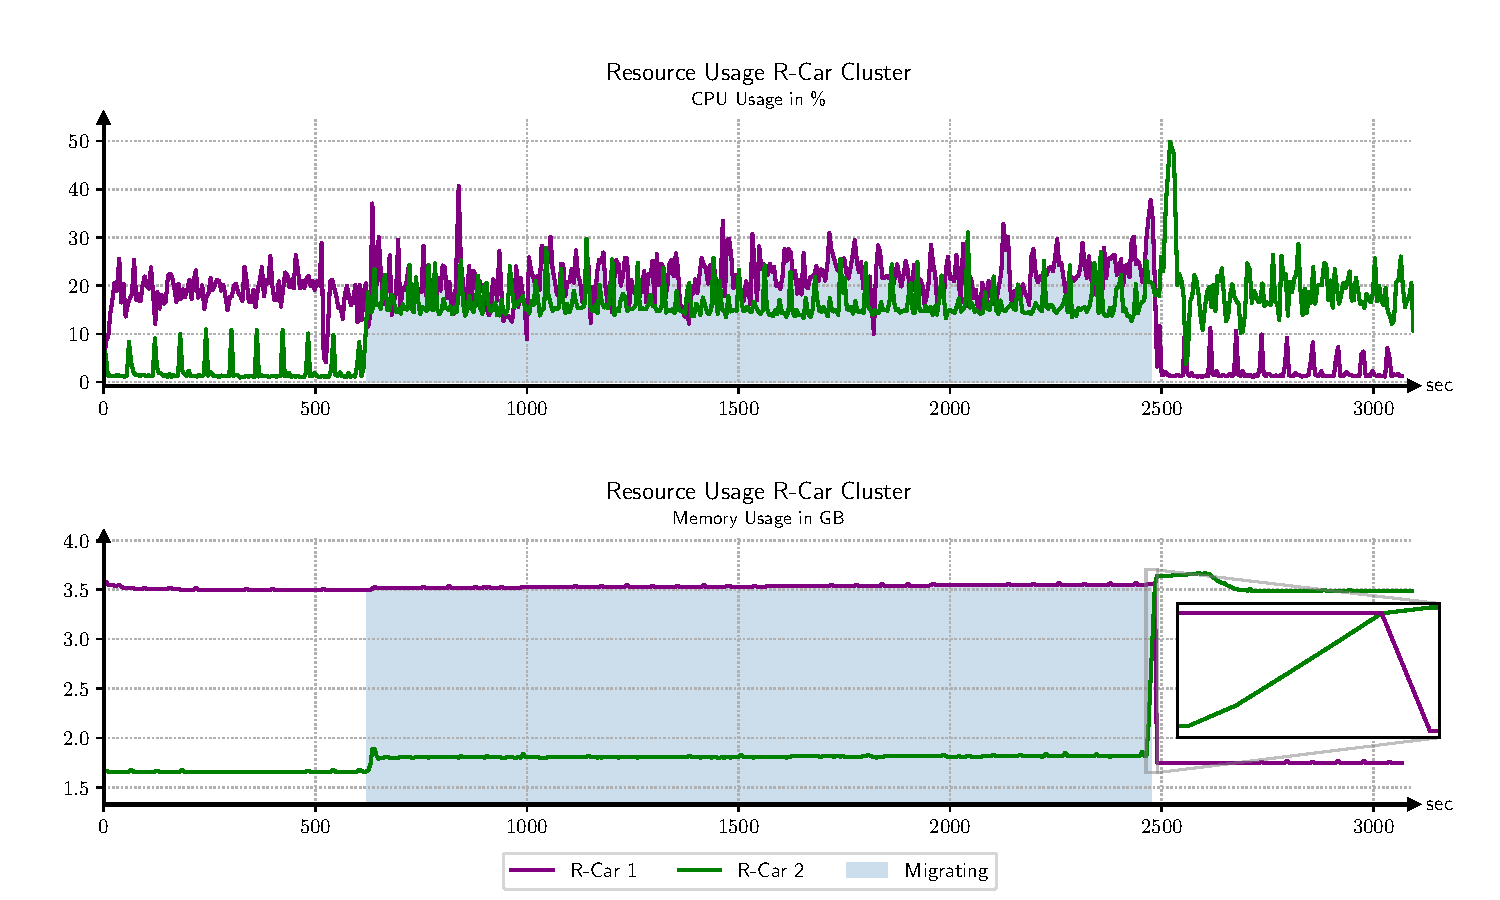
\includegraphics[width=\textwidth]{06_use-case-migration-rcar.pdf}
                \end{subfigure}
                \begin{subfigure}[b]{0.93\textwidth}
                    \centering
                    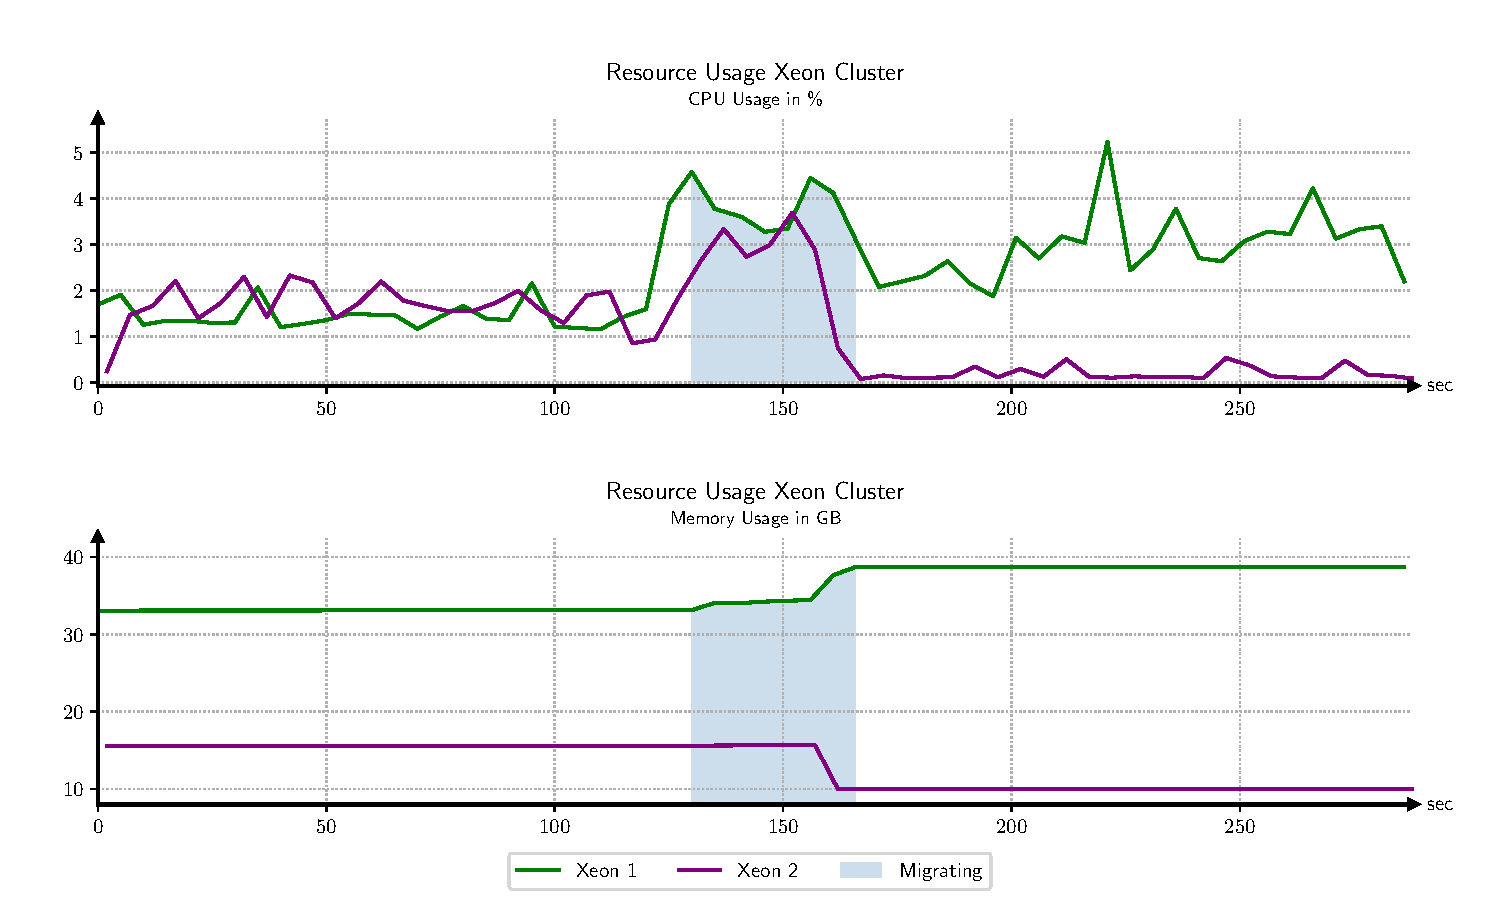
\includegraphics[width=\textwidth]{06_use-case-migration-xeon.pdf}
                \end{subfigure}
                \caption{R-Car and Xeon resource usage with VM application and migration}
                \label{figure:use_case_migration}
            \end{figure}
            
            \noindent The Xeon cluster, on the other hand, shows noticeable better and more confident results.
            Comparing the migration duration with results from Section \ref{subsection:usecases_time}, the times only differ slightly.
            While the idle \ac{VM} needs 34 seconds, the \ac{VM} with an active application takes only 3 seconds or 8\% longer.
            As on the R-Car cluster, Figure \ref{figure:use_case_migration} shows the host's additional \ac{CPU} and memory usage during the migration.
            However, contrary to the R-Car cluster, the live-migration affects the destination host and the source host on the Xeon cluster.
            As the migration happens significantly faster on the Xeon cluster, the \ac{CPU} has more load, which explains the not existing \ac{CPU} usage increase on the R-Car cluster.
            Due to the long duration, the R-Car \ac{CPU} can process all instructions over a longer period of time, leading to a lower overall load.
            Also, the increased fundamental \ac{CPU} and memory load through the control services is visible.
            
            \begin{figure}[H]
              \centering
              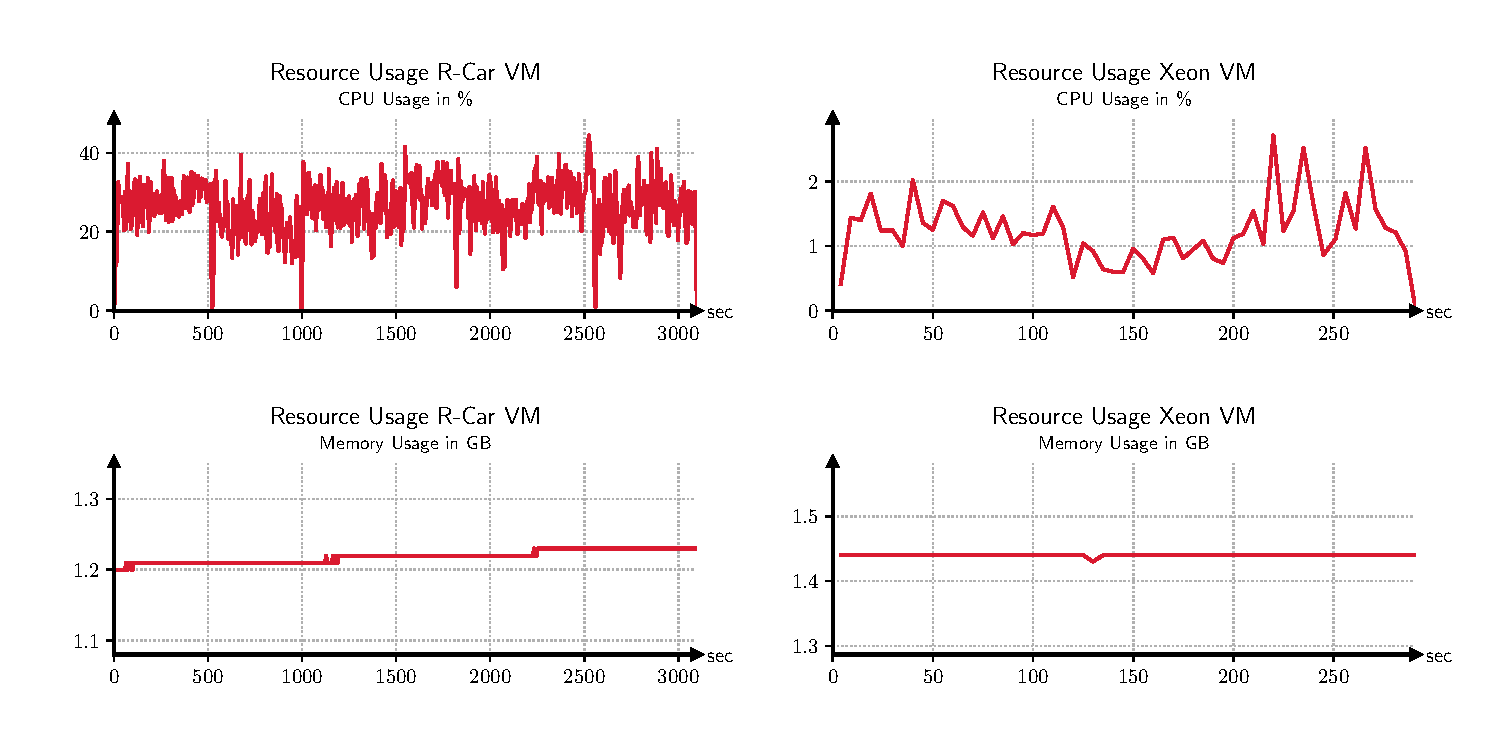
\includegraphics[width=\linewidth]{06_use-case-migration-vm.pdf}
              \captionof{figure}{VM resource usage with VM application and migration}
              \label{fig:use_case_migration_vm}
            \end{figure}
            
            \noindent Finally, Figure \ref{fig:use_case_migration_vm} additionally shows the \ac{CPU} and memory usage of the migrated \acp{VM}.
            The plots show no visible increase in \ac{CPU} or memory usage.
            This underlines that the live-migration does not affect the resource usage inside the \ac{VM}, but only on the host.
            
            \noindent In summary, the R-Car cluster results clearly show the unsuitability for a live- migration in a host failure case.
            Due to the very long duration, the host would have most probably already failed before the complete \ac{VM} would be fully migrated.
            On the Xeon cluster, on the other hand, the migration time is significantly lower.
            Also, the used \ac{VM} flavor represents an improbable \ac{VM} configuration, indicating even lower migration times using smaller \ac{VM} flavors.
            Therefore, the results suggest actual usability of the live-migration functionality if the hardware is powerful enough.
            
    \section{Summary}
        
        \noindent Concluding from the two examined use cases, OpenStack's advantages can be exploited.
        On both platforms evaluated, the tested functionality is reliably and continuously available.
        However, the smaller resources on the R-Car nodes along with the not advantageous big.LITTLE architecture and slow-performing SD-Card, counteract a performable operation of OpenStack.
        While the performance doesn't influence the VM distribution, VM migration is greatly influenced.
        As migration times with idle VMs seem to be just in an acceptable range, further measurements show the influence of active VMs on the migration time.
        With migration times spanning multiple minutes up to half an hour, this is not practicable in a real-world scenario and therefore doesn't introduce additional value.
        Powerful hardware, in contrast, is able to perform the migration in reasonable time frames, even with very large VMs.
        This allows the assumption that also the ARM platform would achieve better results with more resources available.
        Figure \ref{figure:use_case_migration} depicts that more memory, for example, 8 or 16 GB, could already suffice to achieve reasonable migration times.
        Together with more cores to provide adequate resources to the host and guest system and as well as faster storage better performance could most probably be achieved.
        
        
        
        
        
        
